\documentclass{article}

\usepackage[margin=3cm]{geometry}
\usepackage{graphicx}
% \usepackage{subfigure}
\usepackage{caption}
\usepackage{subcaption}
\captionsetup[table]{skip=0pt}
% \usepackage{url}
\usepackage{hyperref}
\usepackage{hhline}

\usepackage{algorithm}
\usepackage{amsmath}
\usepackage{ bbold }
\DeclareMathOperator*{\argmin}{arg\,min}


\title{Simulated Annealing Algorithm for Graph Coloring\\Random Walks course project}
\date{May 25, 2016}

\author{
  R\'oger Berm\'udez Chac\'on\\EPFL
  \and
  Victor Kristof\\EPFL
  \and
  Merlin Nimier-David\\EPFL
}

\begin{document}
  \maketitle

  \paragraph{Abstract}
  We formulate the graph coloring problem as an optimization problem and use the Markov Chain Monte~Carlo method to find proper colorings. Simulated annealing is used to improve the convergence speed and avoid local minima. In this report, we recall the problem statement and formulation, describe the simulated annealing schemes devised and present results.

  % -----------------------------------------------------------------------------------
  \section*{Problem statement}
  \paragraph{Proper $q$-colorings}
  Let $G = (V, E)$ a graph with $|V| = N$ vertices. A \emph{coloring} using $q$ colors is an assignment $x \in \{ 1, \ldots, q \}^N$ for all elements in $V$. A \emph{proper} $q$-coloring is a coloring such that no two adjacent vertices have the same color: $(v, v') \in E \Rightarrow x_v \neq x_{v'}$. From this definition, we can define a cost function (Hamiltonian) to evaluate the ``quality'' of a given coloring:
  \[
    H(x) = \sum_{(v, v') \in E} \mathbb{1}_{x_v = x_{v'}}.
  \]

  In the general case, finding the proper $q$-coloring of a graph of size $N$ is NP complete\footnote{\url{https://en.wikipedia.org/wiki/Graph_coloring\#Computational_complexity}}, assuming $2 < q < N$. The search space is the domain of all colorings $x$, which has a size exponential in $N$. It is therefore interesting to relax the problem into an optimization problem. Using the cost function defined above:
  \[
    x^* = \argmin_{x \in \{ 1, \ldots, q \}^N} H(x).
  \]
  We have, then, that $x^*$ is a proper coloring when the minimum cost achieved is $0$. In the following section, we will describe how the Metropolis-Hastings algorithm can be used in this setting.

  \paragraph{Input data}
  In this project, we use Erd\H{o}s-R\'{e}nyi random graphs to test the correctness of our implementation and convergence speeds. They are constructed as follows: for a given density parameter $c$, each pair of the $N$ vertices is connected with probability $c / N$. Examples are given in Figure~\ref{Fig:random-graph-examples}, where an initial random coloring is also visualized.

  \begin{figure}[h]
      \centering
      \begin{subfigure}[t]{4.5cm}
        \centering
        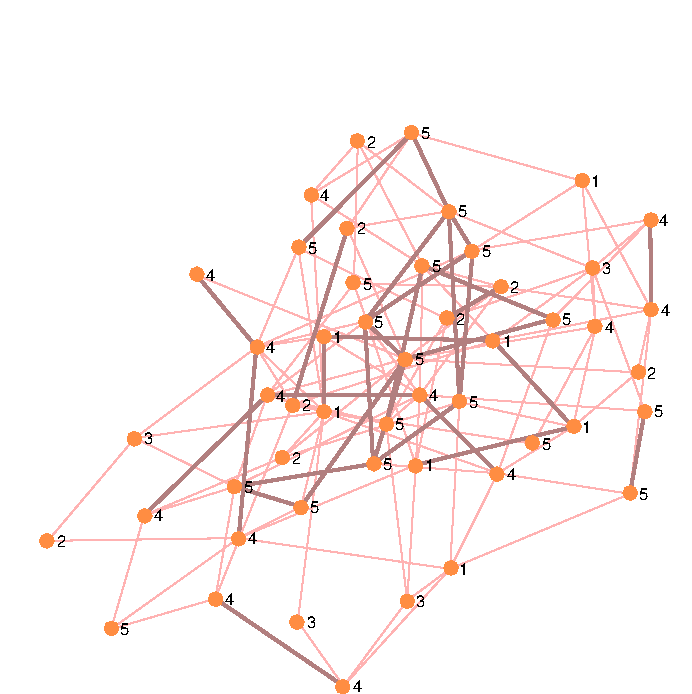
\includegraphics[width=4.5cm]{figures/random-graph-50-5-5.pdf}
        \caption{$c = 5$}
      \end{subfigure}
      \quad
      \begin{subfigure}[t]{4.5cm}
        \centering
        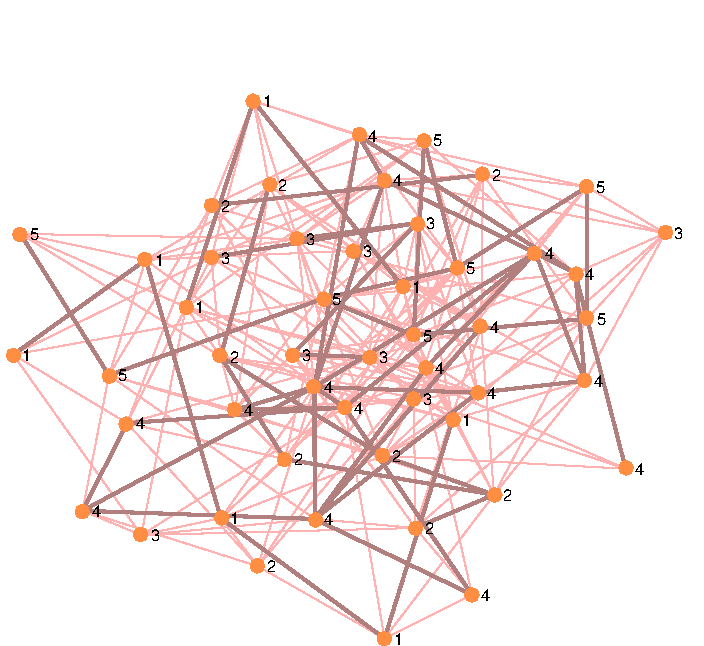
\includegraphics[width=4.5cm]{figures/random-graph-50-10-5.pdf}
        \caption{$c = 10$}
      \end{subfigure}
      \quad
      \begin{subfigure}[t]{4.5cm}
        \centering
        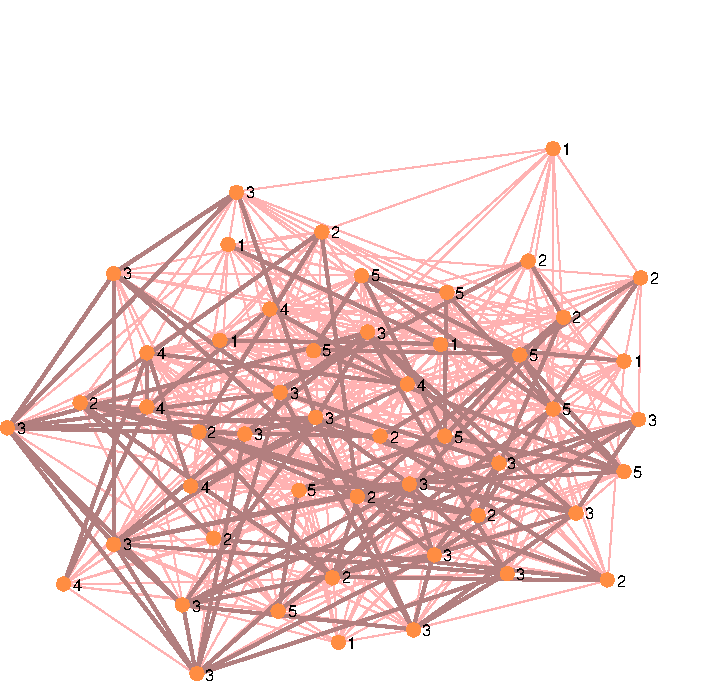
\includegraphics[width=4.5cm]{figures/random-graph-50-20-5.pdf}
        \caption{$c = 20$}
      \end{subfigure}

    \caption{Examples of Erd\H{o}s-R\'{e}nyi random graphs ($N = 50$ edges) for different values of the density parameter $c$. We also visualize an initial random coloring: numbers next to the edges represent their colors; improper vertex colorings are shown in bold.}\label{Fig:random-graph-examples}
  \end{figure}

  % -----------------------------------------------------------------------------------
  \section*{MCMC solution}
  Once the graph coloring problem is formulated as an optimization problem, we are able to bring it into the MCMC framework. We setup a simple Markov Chain over the space of colorings. Transitions correspond to changing one vertex (chosen uniformly at random) to a different color (chosen uniformly at random). After generating a proposed transition, we compute the change in cost:
  \[
    \Delta = H(x^{new} - H(x^t).
  \]
  The proposed transition is performed with some acceptance probability, defined below. This process is repeated until a proper coloring is found ($H(x) = 0$) or a maximum number of iterations is reached.

  Figure~\ref{Fig:random-walk-example} shows the evolution of cost $H(x)$ over the course of an example walk. When enough colors $q$ are available w.r.t. the density $c$ of the graph, the walk converges to a proper coloring in few iterations. We plot in Figure~\ref{Fig:cost-vs-density} the relationship between the best cost achieved and the graph's density, for different values of $q$.

  \begin{figure}[h]
    \centering
    \begin{subfigure}[t]{.49\linewidth}
      \centering
      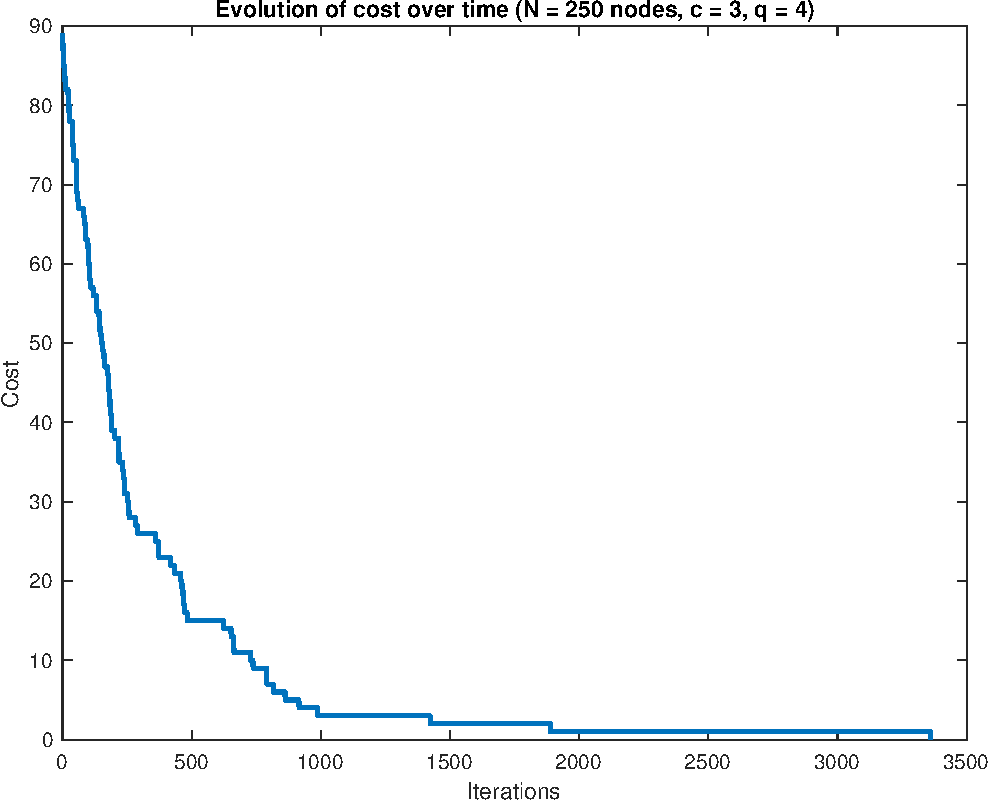
\includegraphics[width=.8\linewidth]{figures/random-walk-example.pdf}
      \caption{}\label{Fig:random-walk-example}
    \end{subfigure}
    \begin{subfigure}[t]{.49\linewidth}
      \centering
      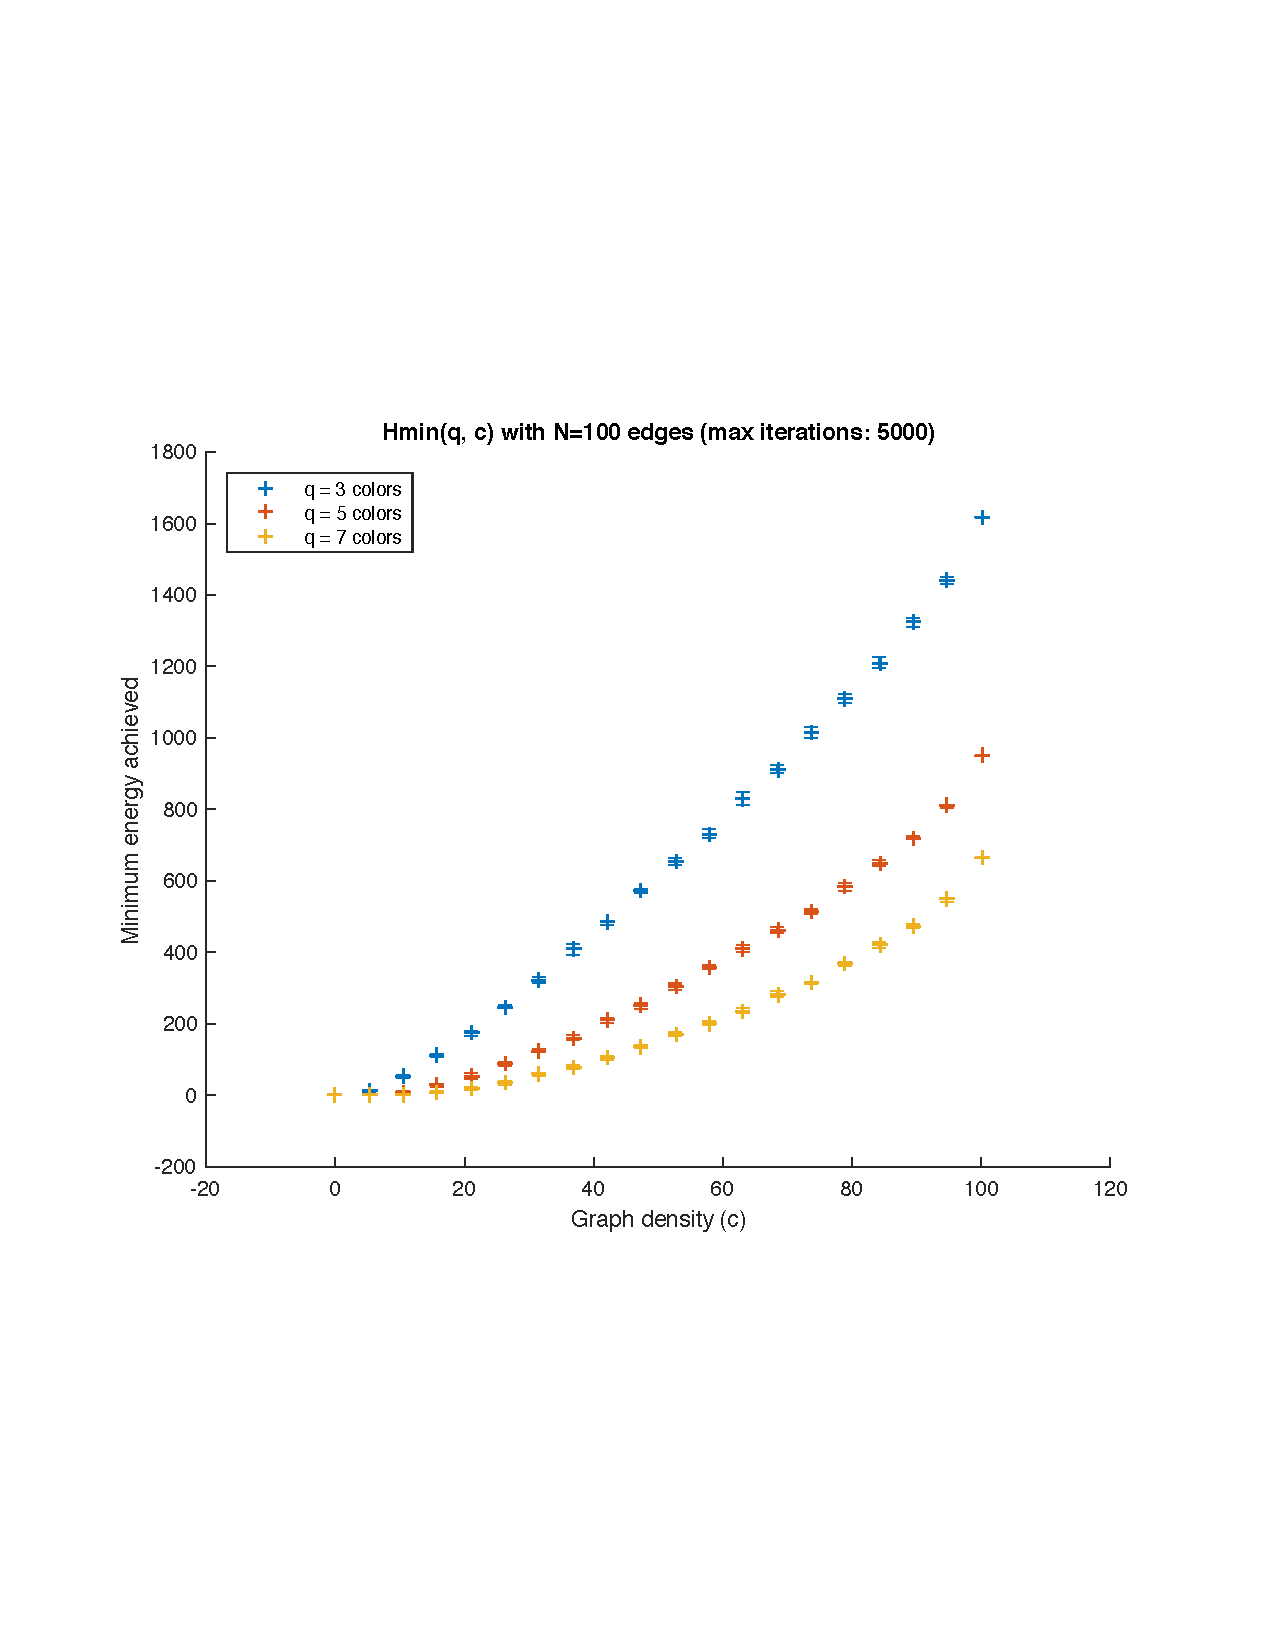
\includegraphics[width=.8\linewidth]{figures/cost-vs-graph-density.pdf}
      \caption{}\label{Fig:cost-vs-density}
    \end{subfigure}
    \caption{Left: evolution of the cost over time for an example graph. Right: minimal energy achieved as a function of graph density $c$ for different values of $q$. Since both the input data and the process are random, we perform the optimization for $5$ random inputs for each set of parameters and show error bars.}
  \end{figure}

  \paragraph{Simulated annealing}
  In order to find the global minimum of our cost function $H(x)$ that potentially contains several local minima, we make use of the \textit{simulated annealing}. This method simulates the physical process of cooling a solid such that when its structure is frozen, the minimum energy configuration is reached. During the cooling procedure, we reduce the ``temperature'' $T$ or, equivalently, increase the ``inverse temperature'' $\beta=\frac{1}{T}$. The way the temperature is reduced is managed by a ``schedule'', a function of the current time step. In our implementation, we perform simulated annealing by increasing $\beta$ and the schedule will be referred to as $\beta(t)$. The acceptance probability for a proposed move with energy difference $\Delta$ is defined as:
  \[
    p = \exp(- \beta(t) \times \Delta).
  \]

  % -----------------------------------------------------------------------------------
  \section*{Results}
  % This paragraph is not so important, since we don't have a lot of space
  % \paragraph{Implementation details}
  % TODO: Efficient implementations for generating the graph, transitioning, etc. Give some number to describe algorithm's performance (e.g. average time / iteration). Point out what can be parallelized (several independent chains with different initializations can run in parallel) and what cannot (a single chain).

  % \paragraph{Experiments}
  We define in Table \ref{tab:schedules} five different schedules, each tunable by some parameters. They all depend on the current time step $t \in [0, 1]$, normalized by the maximum number of iterations. The inverse temperature $\beta(t)$ should approach ``infinity'' when $t$ approaches the maximum number of iterations, such that the acceptance probabilities approach $0$ at this time. Moreover, in each case, a time delay $\tau$ can be introduced ($t$ becomes $t-\tau$) in order to keep $\beta(t)$ constant at the beginning of the simulation before starting to increase it. However, in most cases, we don't notice an increase in the performances by doing so.

  \begin{table}[h]
    \begin{center}
    \def\arraystretch{1.5}
      \begin{tabular}{|c||c|c|c|c|c|}
      	\hline
        \textbf{Schedules} & \textbf{Linear} & \textbf{Sublinear}  & \textbf{Polynomial}  & \textbf{Logarithmic}& \textbf{Exponential} \\
        \hhline{|=||=|=|=|=|=|}
        \textbf{$\beta(t)$} & $\beta_0 + \alpha t$ & $\beta_0 t^{\alpha}$, $\alpha < 1$ & $\beta_0 t^{\alpha}$, $\alpha > 1$& $\beta_0 \log (t + \alpha)$, $\alpha \geq 1$ & $\beta_0\alpha^{-t}$, $0 < \alpha < 1$  \\
      	\hline
	\textbf{Parameters} & \begin{tabular}[t]{@{}c@{}}$\beta_0=0.001$ \\ $\alpha=6$\\$\tau=0.05$\end{tabular} &  \begin{tabular}[t]{@{}c@{}}$\beta_0=10$ \\ $\alpha= 0.5$\\$\tau=0$\end{tabular} &  \begin{tabular}[t]{@{}c@{}}$\beta_0=10$ \\ $\alpha=2.5$\\$\tau=0$\end{tabular} &  \begin{tabular}[t]{@{}c@{}}$\beta_0=10$ \\ $\alpha=1$\\$\tau=0$\end{tabular} &  \begin{tabular}[t]{@{}c@{}}$\beta_0=0.01$ \\ $\alpha=0.0005$\\$\tau=0$\end{tabular} \\
	\hline
      \end{tabular}
    \end{center}
    \caption{Schedules for $\beta(t)$. The parameters are hand-tuned.}
    \label{tab:schedules}
  \end{table}

  We hand-tune the parameters of each schedule in order to obtain good results. The shape of the schedules are shown in Figure \ref{fig:schedules_shape}. We then compare them against each other on a graph of size $N=250$ and using $q=15$ colors. The edges density $c$ is linearly increased from 0 to $N/4$. The results are displayed in Figure \ref{fig:schedules_evaluation}. The sublinear schedule (here, a square root) performs consistently better than the others. We notice that the logarithmic schedule, also a slow-growing function of time, has similar performance.

  \begin{figure}[h]
    \centering
    \begin{subfigure}[t]{.5\linewidth}
      \centering
      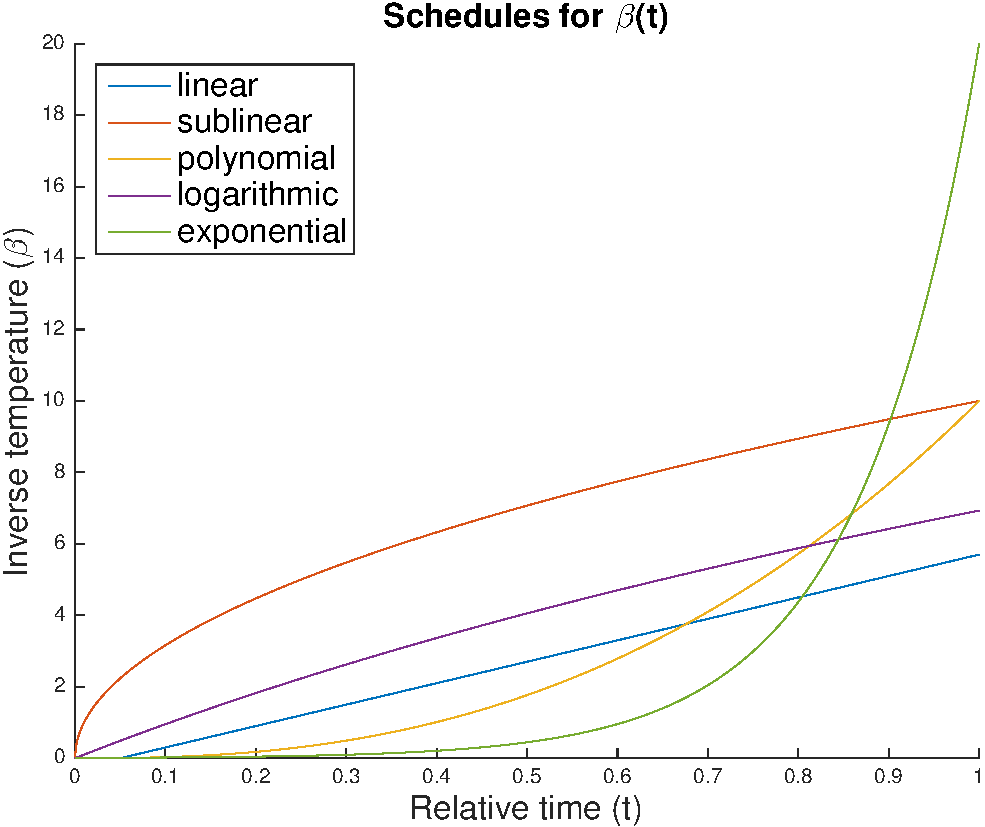
\includegraphics[width=.8\linewidth]{figures/schedules_shape.pdf}
      \caption{Shape of the schedules described in Table \ref{tab:schedules}.}
      \label{fig:schedules_shape}
    \end{subfigure}%
    \begin{subfigure}[t]{.5\linewidth}
      \centering
      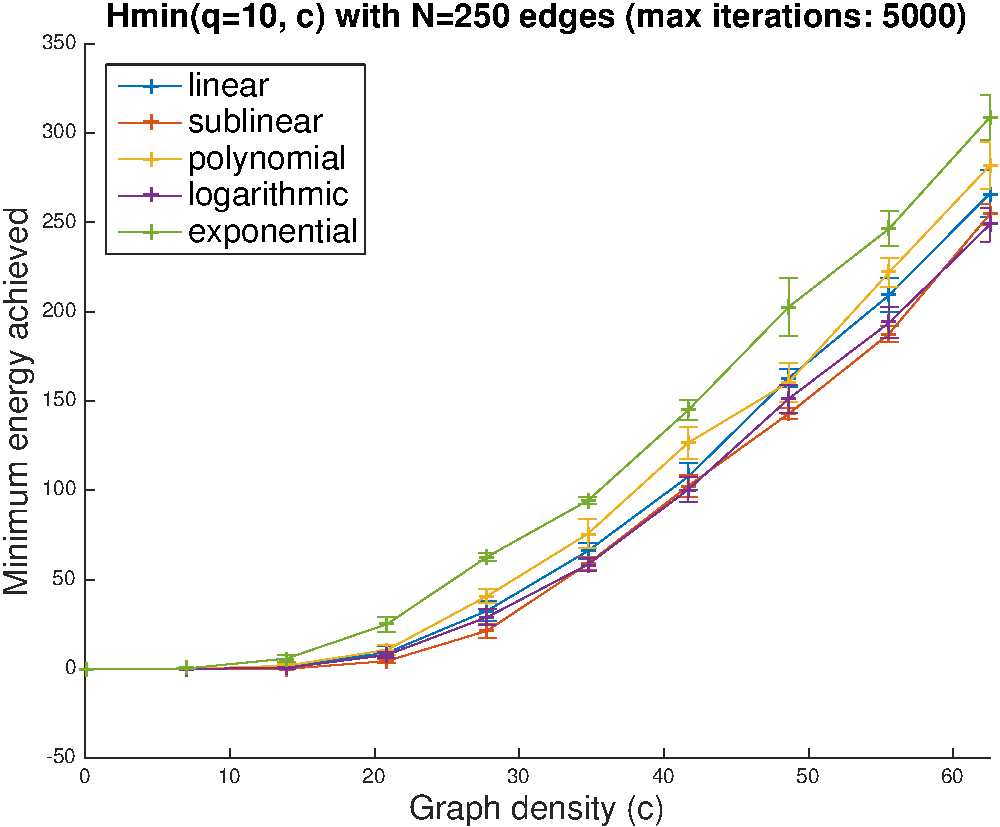
\includegraphics[width=.8\linewidth]{figures/schedules_evaluation.pdf}
      \caption{Results of the graph coloring on a graph of size $N=250$ and with $q=10$ colors. The ``square root'' schedule performs best.}
      \label{fig:schedules_evaluation}
    \end{subfigure}
    \caption{Shape of schedules and comparison against each other.}
    \label{fig:schedules}
  \end{figure}

\end{document}

